\documentclass[11pt,a4paper]{report}

\usepackage[margin=1in]{geometry}
\usepackage[utf8]{inputenc}
\usepackage[T1]{fontenc}
\usepackage{graphicx}
\usepackage[dvipsnames,table]{xcolor}
\usepackage[colorlinks=true, linkcolor=NavyBlue, urlcolor=NavyBlue]{hyperref}
\usepackage{colortbl}
\usepackage{booktabs}
\usepackage{tabularx}
\usepackage{float}
\usepackage{enumitem}
\usepackage{longtable}
\usepackage{amsmath, amssymb}
\usepackage[most]{tcolorbox}
\usepackage{titlesec}
\usepackage{fancyhdr}
\usepackage{microtype}

\setlist[itemize]{nosep, leftmargin=*, topsep=2pt, partopsep=0pt}
\setlist[enumerate]{nosep, leftmargin=*, topsep=2pt, partopsep=0pt}
\widowpenalty=10000
\clubpenalty=10000
\brokenpenalty=10000

\definecolor{acc}{HTML}{1F4E79}
\definecolor{warn}{HTML}{9C4221}
\definecolor{good}{HTML}{2F6042}
\definecolor{soft}{HTML}{F2F5F9}

\titleformat{\chapter}[display]
  {\normalfont\huge\bfseries\color{acc}}{\chaptertitlename\ \thechapter}{12pt}{\Huge}
\titlespacing*{\chapter}{0pt}{-10pt}{24pt}
\titleformat{\section}{\large\bfseries\color{acc}}{\thesection}{0.7em}{}

\pagestyle{fancy}
\fancyhf{}
\lhead{\small\leftmark}
\rhead{\small\thepage}
\renewcommand{\headrulewidth}{0.4pt}

\newtcolorbox{evidence}[1][]{colback=soft, colframe=acc!70, fonttitle=\bfseries,
  boxrule=0.6pt, left=6pt, right=6pt, top=5pt, bottom=5pt, breakable, #1}
\newtcolorbox{caution}[1][]{colback=warn!5, colframe=warn!70, fonttitle=\bfseries,
  boxrule=0.6pt, left=6pt, right=6pt, top=5pt, bottom=5pt, breakable, #1}
\newtcolorbox{resolved}[1][]{colback=good!5, colframe=good!70, fonttitle=\bfseries,
  boxrule=0.6pt, left=6pt, right=6pt, top=5pt, bottom=5pt, breakable, #1}

% float placement: let tables share pages with text instead of stranding
\setcounter{topnumber}{2}
\setcounter{totalnumber}{3}
\renewcommand{\topfraction}{0.9}
\renewcommand{\bottomfraction}{0.7}
\renewcommand{\textfraction}{0.1}
\renewcommand{\floatpagefraction}{0.8}

\newcommand{\keyrule}[1]{\textbf{\textcolor{acc}{#1}}}

\title{\vspace{-2em}\textbf{The RPent Harness}\\[0.4em]
\large From the upstream project to a self-growing system:\\
architecture, history, experiments, and what the evidence supports}
\author{RPent harness project}
\date{12 August 2026}

\begin{document}
\maketitle

\begin{abstract}
\noindent
This document records a rebuild. A LIBERO manipulation benchmark is driven by a
text-only planner (\texttt{deepseek-v4-flash}) that never sees an image; the
work described here is the harness around that fixed, cheap model --- the tool
layer it acts through, the boundary it acts inside, the record it leaves, and
the mechanism by which it accumulates knowledge between runs.

The account is in build order, because each layer exists to make the next one
measurable. It ends with four experimental arms, one controlled ablation, and a
section of equal length devoted to claims this project made and then had to
retract. That last part is not modesty. The central assertion here is that a
harness is worth building only if it can tell you what it is worth, and a
project that cannot catch its own errors has not demonstrated that.
\end{abstract}

\tableofcontents

% ==========================================================================
\chapter{Orientation}

\section{The system in one page}

Three GPU services run behind an HTTP boundary: a MuJoCo environment, a frozen
Pi0.5 vision-language-action policy, and SAM 3.0 for segmentation. In front of
them sits a planner --- a language model in a turn loop --- which issues tool
calls and reads their results. The planner is blind by construction. It is
launched with \texttt{-{}-no-images} and receives no pixels; segmentation
results, world-coordinate maps and geometric measurements are its entire access
to the scene.

That constraint is deliberate and it shapes everything downstream. A blind
planner must \emph{measure} rather than look, which means every belief it holds
about the world traces to a tool result, which means the run's record can be
audited for whether a decision was earned or invented. The project's governing
rule follows from that: heavy data stays on disk and references travel in
context. Point clouds and images never enter the prompt; tools read paths,
compute, and return numbers the planner reasons over and cites.

\section{Two rules that settled most arguments}

\keyrule{Mechanism over discipline.} A rule written into a prompt is discipline; a
gate in the tool-dispatch path is mechanism. Wherever both were possible,
mechanism won. The clearest case is the sandbox (Chapter~\ref{ch:sandbox}): three standing
prohibitions in the prompt became one allowlist in code, and the prompt then
stopped mentioning the forbidden files at all --- because naming a file in order
to forbid it advertises that it exists.

\keyrule{Attribution is the point.} The purpose of the infrastructure is to be able
to say what a component is worth: in points, in tokens, and when it is harmful.
Decisions were judged against whether they made attribution easier. This is why
the middleware order is a declared constant, why every run writes a fingerprint
of the boundary it ran under, and why the experiments in Chapter~\ref{ch:exp} are
organised around a single-variable comparison rather than a headline number.

\section{What changed, at a glance}

The branch point is upstream \texttt{RLinf/RPent} at commit \texttt{3c2516e3}.
Against it, this work is roughly sixty commits over 120 files.

\begin{table}[htbp]
\centering\small
\begin{tabularx}{\textwidth}{@{}l X@{}}
\toprule
\textbf{Layer} & \textbf{Change} \\
\midrule
Tools & one 1{,}930-line module becomes a package of 15; hand-written schema dicts become native framework tools; five-hop dispatch becomes two \\
Descriptions & every word the model reads about a tool moves into one structured, linted source \\
Prompt & per-cell answers deleted; then the prompt is made to vary with the sandbox's capabilities rather than its name \\
Sandbox & always-on, fail-closed file boundary; profiles as data; the priors download becomes opt-in and staged \\
Evidence & every tool call recorded including read-only ones; an append-only entity databus; replay rebuilt from disk artifacts alone \\
Gate & a five-check promotion pipeline with a human interrupt, the only writer of the memory library \\
Regimes & practice and exam seeds separated in code; experiment episodes; resident multi-attempt debugging sessions \\
Perception & a queryable vision instrument, added as a tool rather than a model swap \\
\bottomrule
\end{tabularx}
\end{table}

% ==========================================================================
\chapter{The starting point}

The upstream harness worked, and two of its properties were judged good enough
to preserve rather than redesign: perception and action are separated, and
privileged information is withheld in code rather than requested politely in the
prompt. The instruction taken from the project owner was to wrap and extend that
layer, not restructure it.

What needed changing was different in kind. \texttt{robots/libero/tools.py} held
1{,}930 lines containing motion primitives, the policy bridge, segmentation,
geometry, state dumping and hand-written tool-schema dictionaries in one
namespace. A call reached its implementation through a five-hop chain: registry
lookup, spec dictionary, name string, attribute lookup, partial application,
handler. Nothing was wrong with any single hop. The problem was that five hops
offer five places to forget a cross-cutting concern, and every mechanism in this
document is a cross-cutting concern.

Alongside the code sat the real obstacle to measurement. The prompt contained
per-task recipe blocks with coordinates for tasks t0 through t9. A calibration
guide of 187 numeric constants was injected on every run. And a resources
directory containing per-cell solutions was re-downloaded and overwritten from a
model hub \emph{on every run}, which meant deleting the answers locally did not
make them go away.

\begin{caution}[title={The measurement this made impossible}]
Counted from the logs afterwards: of 155 runs in that era, \textbf{104 read a
per-cell answer file} for the cell they were being scored on, and 89 read the
calibration table. No number produced in that period measures a harness. It
measures a lookup.
\end{caution}

% ==========================================================================
\chapter{The tool layer}

\section{From one module to a package}

The module became fifteen files split by tool kind: geometry, state, perception,
motion, the policy bridge, schemas, descriptions, context, the databus, the
artifact layout, and a small dependency-free catalogue. Total lines rose from
1{,}930 to 4{,}481, and that arithmetic deserves honesty --- it is not a pure
split. Six of the fifteen modules are concerns that did not previously exist as
code at all.

Tools are now native framework tools: a decorator, a typed argument schema, and
a runtime parameter carrying the live context. A complete tool is short enough
to read whole.

\begin{evidence}[title={A tool, start to finish}]
\ttfamily\footnotesize
@tool(args\_schema=Pi0PickInput, description=tool\_docs.render\_description("pi0\_pick"))\\
def pi0\_pick(prompt, runtime, max\_chunks=24, lift\_thresh=0.05, ...):\\
\hspace*{2em}"""Model-facing text renders from tool\_docs --- edit it there."""\\
\hspace*{2em}ctx = \_context(runtime)\\
\hspace*{2em}return ctx.advance("pi0\_pick", \{...\}, ctx.primitives.pi0\_pick)
\end{evidence}

\noindent
Dispatch is two hops: the tool function, then \texttt{ctx.advance}, then the
primitive. No name-string lookup, no partial application, no dispatch table.

\section{Why this is not cosmetics}

\texttt{ctx.advance} becomes the single seam that every
environment-advancing call passes through, and it owns all the per-action
bookkeeping: timing, cancellation, the action-video slice, the step counter, the
staleness downgrade in the databus, the state dump, and rendering the new state
back to the planner. No tool reimplements any of it and no tool can forget it.

That single seam is what later makes the evidence layer, the attempt rotation
and the sandbox's write protection possible \emph{as mechanisms} rather than as
conventions. It is also where a defect found by the evidence layer was fixed: a
finished episode cannot step again, and rather than crash, the seam now returns
an explanatory error, because experiment episodes routinely keep probing after
an accidental solve and one late call must not cost a run its notes.

The vocabulary of ``which calls mutate the world'' lives in a 32-line module
that imports nothing, and it cannot drift: the tool module raises at import time
if its own advancing-tool list disagrees with the catalogue.

\section{Three decisions worth recording}

\keyrule{Never add postponed annotation evaluation to the tool module.} The
framework detects the runtime parameter by resolving its annotation to a real
type. Under postponed evaluation it sees a string, injection silently fails, and
every tool call dies \emph{at dispatch, not at import}. Every other module in
the repository has that import, so this is precisely what a tidy-up commit
``fixes''.

\keyrule{Schemas are typed models, and that was a reversal.} The first adapter
passed the existing schema dictionaries through unchanged so the model-facing
surface could be \emph{proven} identical across the migration. The owner
reversed it: one definition should give validation, schema and types together.
The cost was accepted explicitly --- the rendered schema shape changed, so the
equality proof was void.

\keyrule{Two namespaces, both names correct.} Nine of fourteen tools wrap mixin
methods, and the decorator cannot decorate a method. Collapsing the namespaces
would have forced renaming every physics function so the tool could own the good
name. Five tool names collide with their handlers, which is why the module
imports its siblings as namespaces rather than importing their members.

\section{Convergence with upstream}

Upstream has since moved in the same direction independently: a later commit
introduces a per-run state object owning the step trace and artifact storage,
and a decorator marking handlers as read-only so that others capture an
observation by default. That is the same instinct as the advancing/read-only
split arrived at here. The destinations differ, and the difference is the
subject of Chapter~\ref{ch:evidence}: they centralised \emph{state capture}; this work
centralised the \emph{evidence record}, including the calls that change nothing.

% ==========================================================================
\chapter{One source for everything the model reads}

Everything the model is told about a tool lives in two files: a structured
description entry, and the argument schema whose field descriptions are part of
the model-facing surface. The Python docstrings are developer notes and say so.

The description template has six fields, and the boundaries between them are the
interesting part. Preconditions may not restate arguments, because arguments are
documented in the schema and nowhere else. Selection guidance may not encode
workflow position, because procedure ordering belongs to the system prompt.
Usage notes may not describe multi-step procedures spanning other tools ---
which, in the template's own words, ``is how recipes creep back into tool
descriptions''. Quantitative caveats must have measurement backing.

Content was migrated verbatim from the pre-existing docstrings: sentences were
moved into fields, not reworded. The reason is that the model-facing surface is
an experiment variable, so a wording change must be deliberate and measured
rather than smuggled in with a refactor.

The reason for the ceremony is attribution. That surface has to be a
\emph{surface} --- hashable, diffable, lintable --- rather than a scattering of
docstrings. A stdlib-only test keeps it one, with six checks: import-time
validation, a hand-maintained roster so a rename breaks visibly, symmetric
agreement between documented and real tools, a dangling-reference lint, and
byte-identity between the rendered source and both dispatch substrates. The
sixth is the load-bearing one:

\begin{evidence}[title={The prior-leak lint, run over the rendered bytes the model sees}]
\ttfamily\footnotesize
FORBIDDEN\_PATTERNS = [r"resources/", r"results\_\textbackslash w*", r"env\_calibration",\\
\hspace*{6em} r"guides/", r"past recipe", r"memory file", r"memory librar", r"MEMORY\textbackslash .md"]
\end{evidence}

\noindent
One pattern recurs throughout the rest of this document: a capability that
varies with a runtime flag gets its own description entry, never a static
superset. Under \texttt{-{}-no-images} the image tool is swapped for a variant
that advertises the truth rather than promising something it cannot do.

% ==========================================================================
\chapter{The prompt, and the sandbox that made it honest}
\label{ch:sandbox}

\section{Cleansing: the admission rule}

The prompt lost 42\% of its bytes --- from 33{,}463 to 19{,}544 in source ---
and what left is more interesting than the size. Deleted: the per-task recipe
blocks and their coordinates; a hyperparameter section duplicating tool-schema
defaults; a constant of the form \texttt{eef\_y = plate\_y + 0.045}, which
measurement later refuted when the same offset was found ranging over 1.0 to 4.1
centimetres \emph{within a single run}; the workflow step instructing the agent
to read the seed-0 reference, which was the leak channel itself; and the
187-constant calibration table.

The filter was not ``contains a number''. That filter is wrong in both
directions --- a drawer's region bounds are numeric, invariant and not
perceptually recoverable, which makes them knowledge; ``the dark bottle is the
salad dressing'' has no numbers and is pure answer. The rule is two-dimensional.

\begin{table}[htbp]
\centering\small
\begin{tabularx}{0.92\textwidth}{@{}l X X@{}}
\toprule
 & \textbf{varies with the instance} & \textbf{invariant} \\
\midrule
\textbf{a tool can measure it} & never in the prompt --- measure it & at most a check, never a value \\
\textbf{no tool can recover it} & this is the cheat: a cell's answer & \textbf{the only class worth its tokens} \\
\bottomrule
\end{tabularx}
\end{table}

\noindent
What survived: frame conventions, gripper semantics, which primitive threads a
kinematic singularity, the wrist camera's modality weakness, and the definition
of a stalled motion.

\section{Leveling: deleting the advertisements}

Cleansing removed answers. Leveling removed the \emph{advertising}. The prompt
now varies with what the sandbox actually permits, never with a profile name:
the library instructions exist if and only if the library roots are readable,
probed off the live policy object rather than off the command line. A custom
profile that exposes the library gets the instructions automatically, whatever
it is called.

The consequence the owner insisted on is the one that surprises readers.
\keyrule{Every verbal file prohibition was deleted, in every variant.} The old
blocks forbidding the agent to read the solutions or the calibration table were
discipline standing in for a missing mechanism. Once the sandbox exists they
become pure advertisement: naming a blocked file tells the model it exists and
what is in it. The prior-free prompt now reads as though those files never
existed, and a 44-assertion lint enforces exactly that --- a vocabulary of
forbidden strings that must not appear in \emph{any} variant, plus the reverse
direction, that exam variants must not contain the names of the resident-session
tools they do not ship.

The full capability ladder --- no library, library, library plus task playbook,
plus resident regime --- spans 20{,}551 to 21{,}959 rendered characters. Under
7\% of the prompt, which is what makes it a clean attribution axis.

\section{The sandbox}

\keyrule{Always on.} There is no off switch. Debugging without a boundary is a
named profile whose runs self-identify as measuring nothing. Until the policy is
initialised every check fails closed, so a leak is not reachable by forgetting a
flag.

\keyrule{Profiles are data.} Five short YAML files reference placeholders that are
resolved per run. Code never special-cases a profile name, and unknown keys are
fatal.

\keyrule{Config declares intent; code owns invariants.} The set of write-protected
paths is not in the allowed key set --- it cannot be declared in configuration
at all. It is derived from the artifact layout table, so a new artifact kind is
protected by construction rather than by remembering. \emph{An agent that can
rewrite its own evidence log invalidates every attribution claim}, so that
boundary is not configuration. Every shipped profile, including the permissive
one, allows writes only inside the run directory.

\keyrule{The sync is opt-in and staged.} The download that used to overwrite the
resources directory on every run now happens only if the active profile
references the staging root, targets a staging path rather than the live
directory, reuses an existing copy, and --- deliberately --- has no exception
handler, so a partial sync raises instead of continuing. A comparison arm
running on a silently partial payload measures nothing.

\section{Deleting the old memory}

The sandbox is half the story. The library that shipped from the model hub still
contained the refuted constant. Cleansing the prompt had not cleaned the
library. The resolution was not to edit the old library but to stop injecting it
and \textbf{rebuild a new one from zero under gate control}. The current library
holds 21 general entries and a growing set of task-scoped ones, none of which
existed before this work, and every one of which carries the run citations it
was mined from.

\begin{table}[htbp]
\centering\small
\begin{tabular}{@{}l c c c@{}}
\toprule
\textbf{Era} & \textbf{Runs} & \textbf{Read answer files} & \textbf{Read the calibration table} \\
\midrule
Pre-refactor & 155 & \textbf{104 (67\%)} & 89 \\
This framework, before the sandbox & 11 & 1 & 11 \\
This framework, sandbox on & 136 & \textbf{0} & \textbf{0} \\
\bottomrule
\end{tabular}
\caption{The sandbox's acceptance test, counted from run logs.}
\end{table}

% ==========================================================================
\chapter{The evidence layer}
\label{ch:evidence}

\section{Recording the calls that change nothing}

The step trace only gains an entry when a primitive advances the environment. On
one examined run, 27 tool calls happened and the trace held 6. Everything about
perception and file reading --- including whether the agent read an answer ---
was invisible.

A middleware now writes one line per call from the tool-dispatch wrapper, which
is the only seam that sees every call uniformly. Universality is structural
rather than a policy: the hook wraps the dispatcher, so there is no name filter
and no branch on whether the tool advances anything. A crashed tool is logged
and re-raised. The step index is sampled on both sides of the handler, so
\emph{whether a call advanced the environment is computed from the log rather
than declared in it}, and a read-only call is pinned to the state it observed.

The writer never raises --- a missing log line is a smaller loss than a failed
episode --- appends under a lock because a turn's calls run concurrently, and
imports nothing but the standard library, so a diagnostic can read a run without
the agent framework installed.

Middleware order is a declared constant with its rationale attached: \emph{a
different order is a different method, so it is recorded rather than implicit.}
Four of its nine entries are unimplemented and named on purpose, because naming
a known gap is cheaper than rediscovering it.

\section{The entity databus}

Readings of named entities are appended and never rewritten. A mutable ``current
position'' would destroy the provenance that lets a motion cite the reading it
was planned from. Averaging is deliberately not offered: two readings of a
container's near wall have biases that may cancel, but two readings that caught
an object's body and its cap average to a point on neither.

Staleness is computed by the harness and interpreted by the planner. Four
verdicts are assigned from the measured distance to the end-effector's path, and
the docstring states the approximation rather than hiding it --- only the poses
before and after are known, so a policy call that descends and lifts back to
nearly the same point is invisible to the test. \textbf{The verdict is a lower
bound on disturbance}, and ``unverified'' means \emph{not known to have been
disturbed}, never \emph{known to be untouched}.

Conflicts are reported and never resolved. Two differently-named entities within
three centimetres raise a collision warning --- a threshold taken from data,
since real tabletop objects measured six to twenty centimetres apart while one
object's repeated readings agreed to millimetres. The detector states the limit
of its own reach in the same comment: it catches a collision, not a swap, and
two objects at two positions with their labels exchanged are geometrically
self-consistent.

\section{Replay as a completeness test}

Replay rebuilds a finished run as a turn-by-turn timeline \textbf{from the disk
artifacts alone}, and renders its own incompleteness under a heading of
\emph{record gaps}. That constraint is the feature: a gap means the logs are
missing something and the remedy is to record more, not to improve the renderer.

The join between the call log and the transcript is positional with a name
check, and degrades to a warning rather than misattributing reasoning. Renderers
only read; the single permitted derivation is projecting a recorded
world-coordinate onto a recorded camera image by lookup in the stored maps, and
a projection whose error exceeds five centimetres is drawn as a warning line
rather than a confident dot.

\section{What the layer caught}

\begin{itemize}
\item The policy's success flag is false precisely when pre-positioning is good,
      because its predicate requires a ten-centimetre descent. It penalises the
      behaviour the prompt teaches.
\item Gripper width does not detect a grasp: one run held the same width for
      five consecutive steps while the point cloud found nothing below the
      end-effector for the first three.
\item A geometry tool was reporting the tabletop as a grasped object --- of 25
      closed-gripper steps across six runs, twelve were readings of a surface.
\item Mask edge-bleed inflated every extent measurement, in one case sixfold.
\item A comparison tool cannot separate success from failure: across four
      releases the signature was indistinguishable between runs that solved and
      runs that never terminated, because an object perched on a rim registers
      like a seated one. Reported as a negative result and written into the
      tool's own contract.
\end{itemize}

% ==========================================================================
\chapter{The promotion gate}

\section{Layered digestion}

Knowledge reaches the library through five stages: per-run observation that is
blind to the existing library, sweep-wide synthesis that sees everything,
mechanical review, a human interrupt, and application. Observers being
library-blind is what allows support for a claim to be counted from
\emph{independent} discovery rather than from agreement with what is already
written down.

\keyrule{The iron rule against hearsay.} Proposal evidence grounds to citation
tokens resolved straight into the per-call log, never to the observation files,
which are themselves model output. One grammar covers a tool call, an
environment step and an artifact; the resolver dereferences a token into the
actual record and returns the tool name, arguments, status and result, so the
reviewer reads what the record says rather than what the proposal claims it
says. A proposal with no citations is rejected before it is read.

\section{The five checks}

They are five labelled sections of one pass, each tagging its findings by name.

\begin{enumerate}
\item \textbf{Contract} --- every citation must dereference; touching an
      existing entry raises an automatic flag. If anything rejects here the pass
      short-circuits, because an unevaluable proposal would only generate noise.
\item \textbf{Numbers} --- every number in the prose must appear, to rounding
      tolerance, in some cited record, or: \emph{cite the measurement or delete
      the number}.
\item \textbf{Per-cell answers} --- tier-aware. The task tier may name a cell's
      objects, since that is its purpose, but absolute coordinates are flagged
      because they die with the seed. At the general tiers, any token matching a
      real object name in the cited runs is flagged as an answer rather than
      knowledge --- and that vocabulary is \emph{measured from the runs}, not
      hard-coded.
\item \textbf{Scope} --- a cross-environment claim that names the environment is
      probably environment-scoped.
\item \textbf{Deduplication} --- similarity against the library and against
      sibling proposals.
\end{enumerate}

\noindent
Plus a sixth, unnumbered rule that is the epistemics in one line:
\emph{support is counted, not declared.}

\section{The interrupt, and the only writer}

Review emits a verdicts file with two separate fields: the machine's suggestion,
kept as an immutable record, and the human's line, merely prefilled with it.
Application executes strict equality --- anything not literally ``admit'' is
archived with its reasons --- and re-validates the contract before writing.

That application step being the only writer of the library is not a convention
either: every sandbox profile permits writes only inside the run directory, so
the agent physically cannot write to the library. Its proposals go to a
subdirectory for the gate to judge.

Four verbs encode an asymmetric evidence bar --- wide at the door, strict on
tenure, eviction by refutation. Support is derived from the count of distinct
cited runs rather than the declared field; provenance is appended, never
overwritten; and eviction \emph{archives} with a date stamp before removing,
because an eviction is a negative result rather than a deletion.

\section{The generational protocol, and its honest result}

Clean start, sweep, mine, review, apply, repeat. Five generations were run, and
the single-run scores read $4 \to 5 \to 7 \to 6 \to 5$: a growth curve.

\begin{caution}[title={The curve died, and so did its replacement}]
Under repeats the curve vanished. The figure that replaced it --- a $+0.7$-cell
library effect --- died too, once a fresh no-library sweep at current code
scored 6 and exposed the earlier low score as the casualty of a
request-integrity crash that had since been fixed. \textbf{No library tier
produces a measurable suite-wide lift}: no library, promoted memory and blind
task playbooks are indistinguishable at 6.0. Both claims are retired.
\end{caution}

\noindent
What the protocol \emph{did} demonstrate is that the review process itself
improved measurably: across five cycles the number of human repairs needed went
one, four, one, one, and finally zero. And the ledger produced a finding no
other instrument could: reading turned selective in generation two, which
recovered two cells --- and the same selectivity orphaned an anti-spiral entry
that then sat unread while the cell it addressed spiralled.

% ==========================================================================
\chapter{Regimes: practice, exam, residency}

\section{The seed split}

Seeds 51 and above are practice; lower seeds are scoring seeds. Knowledge
learned on a practice seed may enter the library; a scoring seed is examined
once, single attempt, and never learned from. It is enforced at the argument
parser rather than in a document, and the refusal names the reason: a
multi-attempt session on a scoring seed would poison it.

Experiment episodes replace the task brief with a trials-and-conclusion brief:
run controlled trials against one open question, change one variable at a time,
and write conclusions in relative terms that survive a re-randomised scene. Task
playbooks add a cell-scoped tier to the library, mined and gated exactly like
the general tier.

\section{Resident debug sessions}

The owner asked for debugging in the style of a published agent system. The
first build was a between-episode loop, and the owner pushed back twice,
correctly: it was reflect-and-retry, and the reference system debugs
\emph{within} the task. On re-reading, the distinction that matters is that the
reference debugger is a \textbf{resident session} --- one long-context session
per task that writes, executes, reads traces, patches and re-executes inside one
continuous context that remembers every prior attempt. A between-episode loop
summons an amnesiac updater per round.

The owner's insight made it cheap to build: the turn loop is \emph{already} a
live session. Three self-imposed walls blocked residency, and each got a
mechanism.

\begin{table}[htbp]
\centering\small
\begin{tabularx}{\textwidth}{@{}X X@{}}
\toprule
\textbf{Wall} & \textbf{Mechanism} \\
\midrule
Episode boundary equals session boundary & a reset tool, capability-gated \\
Single-attempt regime, right for exams & attempt rotation into an archive directory \\
Context budget & per-attempt folding \emph{with a retrieval channel} \\
\bottomrule
\end{tabularx}
\end{table}

\keyrule{Tool existence is the regime boundary.} The reset tool ships only under the
resident flag, which the launcher refuses on scoring seeds. An exam run cannot
be talked into a reset because the tool is not in its surface. The prompt levels
to match: the resident variant \emph{replaces} the single-attempt block rather
than adding to it, because a prompt that forbids resetting while the tool list
ships a reset tool advertises a false boundary.

\keyrule{Folding is admissible only with retrieval.} Folding tool messages into
digests loses information --- unless every digest is an index entry rather than
a summary. Each folded result becomes one line carrying its citation key, and a
dedicated tool resolves that key into the full archived record. Reading the
archived log directly was considered and rejected: it reads head-first with a
character cap, so reaching call 37 would re-inflate the context with calls 1--36
and defeat the fold.

Two further properties are deliberate. Folding is a per-request view rather than
a state rewrite, so the disk record stays complete and replay sees everything.
And it is the first legitimate compaction in this system: archives are
immutable, so the folded prefix is byte-stable and the provider's automatic
prefix cache stays warm --- unlike mid-list summarisation, which invalidates the
cache from the edit point onward.

Rotation carries evidence weight. The archive is registered write-protected the
moment it is created, because evidence of a failed attempt must survive the
session that produced it. The attempt manifest records the model's own diagnosis
in a field the schema requires to be at least twenty characters: \emph{resetting
without a stated change is a rerun, not debugging.}

% ==========================================================================
\chapter{The vision instrument}

t5 exposed a wall that is neither knowledge nor policy. The discriminating
attribute --- which of two similar containers is the target --- has no measuring
channel. Geometry cannot separate them and segmentation collapses six nouns onto
one location. What that looks like from inside is worth quoting, because it is
what running out of measurable options does to a reasoning model:

\begin{evidence}[title={A blind session, turn 16 and then turns 18--19}]
\small\emph{``Wrist probes on A are all within noise (tomato 0.551, bbq 0.574,
red 0.637, brown 0.602) --- language cannot separate the two sauce bottles.''}

\medskip\ttfamily\footnotesize
turn 17\quad out=35{,}814\qquad turn 18\quad out=44{,}006\qquad turn 19\quad out=52{,}198
\end{evidence}

\noindent
Turns 18 and 19 emitted no text and no tool call, each consuming exactly 8{,}192
output tokens --- the entire generation budget, spent inside the hidden reasoning
channel. The run died at turn 19 of 150. It did not fail at the task; it tried
to settle a perceptual question by thinking.

Vision therefore enters as a \textbf{tool}, not a planner swap and not an
injection --- the pull-shaped form matching the rule that the planner reasons and
tools measure. The design commitments:

\keyrule{Verbatim pipe.} The reply passes through unedited: no summarising, no
filtering, no answer extraction, no truncation.

\keyrule{The exact text sent is recorded.} What the intermediary did is auditable
from the run record alone.

\keyrule{The reader gets zero task context.} One fixed system line and the
planner's question. The reader answers about pixels; it does not know what the
task is, so it cannot smuggle a task decision past the planner.

\keyrule{The answer is an opinion, not a measurement.} The documentation says to
cross-check it geometrically.

\keyrule{Arm gating and sandboxing.} The tool ships only when the channel is armed
--- a blind arm does not ship a tool it cannot honour --- and it is sandboxed,
because otherwise it is a byte-exfiltration channel wearing a question mark.

The thesis is the decoupling itself: reasoning runs on one cheap model,
perception on another, and neither is asked to be the other. The structural
argument is attribution --- a monolithic multimodal model makes the perception
channel unmeasurable because there is no seam. Here the seam is one flag wide
and every crossing of it is a logged call with the image path attached.

Within one session the channel both rescued and misled. A pixel answer
back-projected to table level and the re-pick succeeded; a different pixel
answer back-projected to the height of a milk carton, and when the same view was
re-cropped the reader replied that the object in the centre \emph{was} the milk
carton and no target was visible. That pair is why the admitted rule is a height
sanity check rather than a prohibition.

% ==========================================================================
\chapter{Experiments}
\label{ch:exp}

\section{How a solve is counted}
\label{sec:counting}

Ground truth is the environment's own termination flag as recorded in the step
trace. Three weaker signals are rejected for measured reasons. Not the agent's
audit file, which exists only if the agent calls finish --- a run that solves and
then exhausts its budget would score as a failure, and this has already cost
five real solves across the archive. Not the policy's success flag, which is
false on good grasps and true on air grasps. And not the same key across
codebases: upstream removed the field this project uses and writes a differently
named one inside a different container, so a counter written against one shape
scores the other zero and looks like a result.

\keyrule{Interrupted runs are excluded, not scored.} A run killed mid-flight is a
missing measurement, invalid as a failure and as a solve. Exclusion requires
\emph{both} no natural-exit marker \emph{and} a documented abort. Applying the
test to the whole archive found four candidates; three were excluded and one was
kept, because it had logged its exit reason and then died in cleanup, which
makes its measurement complete. A one-condition rule would have deleted a real
failure and inflated an arm.

\section{The four arms}

\begin{table}[htbp]
\centering\small
\begin{tabularx}{\textwidth}{@{}l l c X@{}}
\toprule
\textbf{Arm} & \textbf{Score} & \textbf{n} & \textbf{Composition} \\
\midrule
Upstream, priors on & \textbf{8/10} & 1 & upstream prompt and planner; \textbf{112 answer-file reads across 10/10 runs} \\
Clean-room, no library & \textbf{6.0} (6,\,6,\,6) & 3 & sandbox on, empty library, 0 prior reads \\
Clean-room + library & \textbf{6.0} (7,\,5,\,6) & 3 & + promoted memory and task playbooks \\
\rowcolor{soft} Full design & \textbf{8.0\,$\pm$\,1.0} (9,\,7,\,8) & 3 & + the vision instrument \\
\bottomrule
\end{tabularx}
\end{table}

\noindent
Upstream's score is purchased, and the receipt is legible in one cell. t5 ---
the cell that cost this project a resident session, an instrument and three
adjudicated library entries --- upstream solved at environment step 2, after
reading that cell's answer file three times, with two identical policy calls and
\textbf{no perception of any kind}. That is not a criticism: with the answers on
disk it is the rational move, and the priors are part of that design. It is the
reason the number cannot be read as a measurement \emph{of a harness}.

\section{The controlled ablation}

Blind library arm versus the same arm with the instrument armed: same sandbox,
same library, same model, same budget, same cells, three passes each. The
instrument flag is the only variable, and nothing else in this project is this
clean.

\begin{table}[htbp]
\centering\small
\begin{tabular}{@{}l c c c l@{}}
\toprule
\textbf{Cell} & \textbf{Blind} & \textbf{Instrument} & \textbf{$\Delta$} & \textbf{Reading} \\
\midrule
t0 & 0/3 & \textbf{3/3} & \textbf{+3} & unpredicted; carries the result \\
t1 & 3/3 & 2/3 & $-1$ & noise \\
t2 & 3/3 & 3/3 & 0 & saturated \\
t3 & 2/3 & 3/3 & $+1$ & noise \\
t4 & 2/3 & 3/3 & $+1$ & noise \\
t5 & 0/3 & 1/3 & $+1$ & the designed target --- moved weakly \\
t6 & 2/3 & 2/3 & 0 & knowledge-bound; predicted indifferent \\
t7 & 3/3 & 3/3 & 0 & saturated \\
t8 & 0/3 & \textbf{3/3} & \textbf{+3} & unpredicted; carries the result \\
t9 & 3/3 & \textbf{1/3} & \textbf{$-2$} & regression, see §\ref{sec:losses} \\
\midrule
\textbf{Suite} & \textbf{6.0} & \textbf{8.0} & \textbf{+2.0} & \\
\bottomrule
\end{tabular}
\end{table}

\noindent
\textbf{The entire suite gain is two cells.} In the records the instrument is
used early and for identity discrimination in all six of those runs --- its
designed role --- but some of its answers there are wrong, and no matched-pair
counterfactual exists. \textbf{No causal claim is made for those two cells.}

\keyrule{Arming is not using.} Three of thirty instrument-arm runs carried the flag
and never called the tool. They are functionally blind runs in the instrument
column, which makes the $+2.0$ a mild understatement of what \emph{using} the
instrument is worth and an overstatement of what \emph{arming} it is worth.

\section{Predictions filed before the numbers existed}

\begin{table}[htbp]
\centering\small
\begin{tabularx}{\textwidth}{@{}X l@{}}
\toprule
\textbf{Prediction} & \textbf{Outcome} \\
\midrule
t5 should move; it is the designed target & \textbf{partly wrong} --- 0/3 to 1/3, and not for the predicted reason \\
t6 unchanged; its wall is knowledge & \textbf{correct} \\
t1, t2, t7, t9 saturated and unchanged & \textbf{wrong for t9} \\
t3, t4 noise-dominated & correct \\
t0, t8: prediction explicitly declined & 0/3 to \textbf{3/3} each --- the entire gain \\
\bottomrule
\end{tabularx}
\end{table}

\noindent
The mechanism model was wrong about \emph{where} the value would appear. It was
built for one cell and predicted irrelevant elsewhere; it barely moved that cell
and carried two others. Declining to predict the two chronic failures was
correct, and the reason they were unpredictable is that nobody had ever
diagnosed why they failed.

One filed commitment had to be applied against its author: the pre-registration
named ``a large suite jump without the target cell moving'' as the single result
to distrust on sight, which is exactly what happened. The rule does not fire,
because the movement is concentrated in two chronic zeros at $+3$ each, which
noise at three samples cannot manufacture --- but it is recorded rather than
quietly dropped.

\section{Where the losses came from}
\label{sec:losses}

Four of the six instrument-arm failures ended with the agent \emph{believing it
had succeeded}. That is not a perception failure or a policy failure. It is a
stopping-and-self-reporting failure, and its cause is the subject of §\ref{sec:5f}.

The regression on t9 is part of it. The pre-registered explanation --- turns
burned on instrument calls --- is refuted by the records: one of the two
failures called the instrument \emph{zero} times, and both used exactly 46 tool
calls. Both picked the correct object with real grasps and stopped early.

% ==========================================================================
\chapter{Two case studies}

\section{t6: a knowledge wall}

Under the clean-room sandbox t6 failed eleven consecutive times, and the
no-library arm still fails it. It is now solved five times in six attempts.

\keyrule{The control arm ran first.} An amnesiac between-episode loop ran five
rounds over 115 minutes and self-terminated with the literal string ``no new
knowledge'': zero solves, two entries admitted. Its last two rounds used the same
playbook the experimental arm would start from, which is what makes the
comparison knowledge-fair. What it \emph{could} do is raise good experimental
questions; what it could not do is form the contrast that solved the cell.

\begin{evidence}[title={The discriminator: same prompt, same cell, one move apart}]
\ttfamily\footnotesize
seq 41 --- pi0\_pick("pick up the flat butter slab")\\
\hspace*{2em}success: \textbf{true}\quad min\_gripper\_opening: \textbf{0.0020}\\[0.4em]
seq 50 --- pi0\_pick("pick up the flat butter slab")\ \ \textrm{\emph{(after one pre-position)}}\\
\hspace*{2em}success: \textbf{true}\quad min\_gripper\_opening: \textbf{0.0394}
\end{evidence}

\noindent
The slab is 40 millimetres. The first pick closed to 2 millimetres --- on air ---
and reported success. The harness's own geometry caught it at the next call, and
the wording of that tool result is why the agent believed the measurement over
the flag: \emph{``the points below the eef are geometry, not a grasped object
\ldots\ gripper width alone cannot tell these apart --- it read the same on steps
that were holding and steps that were not.''}

The model then wrote its own diagnosis into the reset call, and that paragraph
is the argument for residency in one artifact --- a diagnosis, a plan, and a
stated decisive variable, written \emph{between} attempts by the context that
ran the first one:

\begin{evidence}[title={The model's reset reason, verbatim}]
\small\itshape
``Attempt 1 SOLVED \ldots\ (2) pre-position at (0.05, -0.101, 0.15) gripper open
then \textrm{\texttt{pi0\_pick}}(`pick up the flat butter slab') --- real grasp
shows final finger opening 0.039 (pinching the 0.04 slab) vs air grasp 0.002
\ldots\ \textbf{first pick from home air-grasped, so pre-positioning above the
butter is the decisive rung.}''
\end{evidence}

\noindent
Its written notes use the citation format the folding middleware mints ---
adopted unprompted as the model's own note-taking grammar. Two proposals were
mined, both \emph{held} by the contract check, and both approved by a human.
Subsequent seed-0 exams, single attempt with no resident tooling on the surface,
solved 3/3 at environment steps 8, 15 and 7. Cross-seed transfer was
\textbf{2/3}: one seed failed.

\begin{figure}[htbp]
\centering
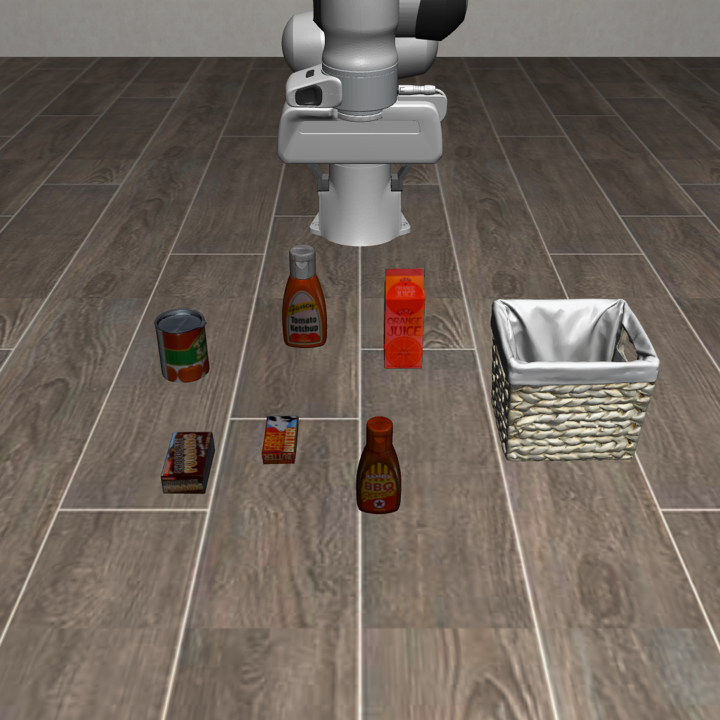
\includegraphics[width=0.47\textwidth]{figures/t6-butter-name-fails.png}\hfill
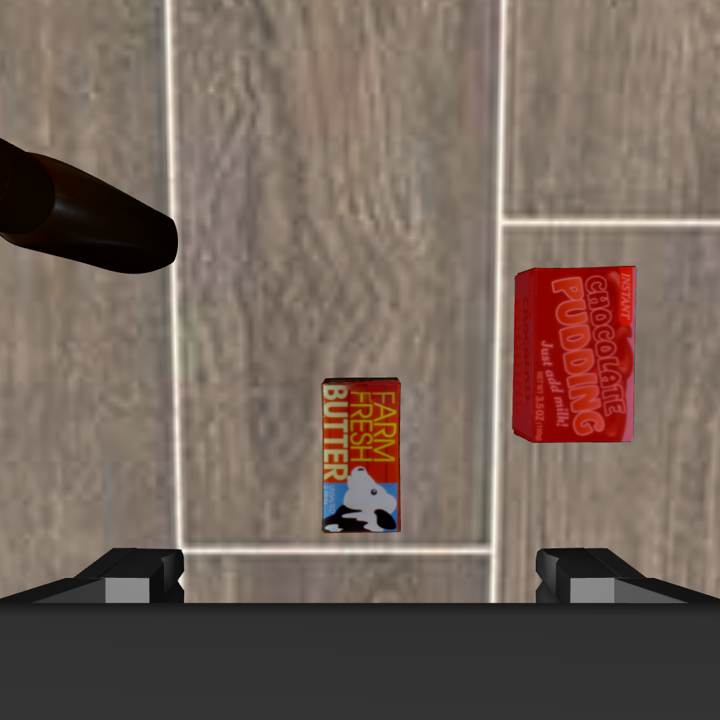
\includegraphics[width=0.47\textwidth]{figures/t6-shape-prompt-fails.png}
\caption[Why t6 needed elimination]{\textbf{Why t6 had to be localised by
elimination.} \emph{Left, agentview:} the prompt \texttt{"yellow rectangular
stick of butter"} (0.562) masks the \textbf{orange-juice carton} --- and returns
the same coordinate as the \texttt{"orange juice carton"} prompt (0.855). The
actual butter is the small flat box lying on the table, centre-left, plainly
labelled, and untouched by the mask. \emph{Right, wrist camera:} a shape-based
phrasing, \texttt{"flat rectangular block on the table"} (0.535), masks the
\textbf{chocolate-pudding box} while \textsc{farm fresh butter} sits unmasked in
the centre of frame.
\textbf{No overlay in this run shows the butter correctly segmented, because no
phrasing ever found it.} The localisation that worked used no segmentation at
all --- an occupancy sweep and a raised-slab discriminator, which produce
numbers rather than overlays. The missing figure is the finding.
Source: \texttt{exam1\_t6\_s0/segments/}, records \texttt{segment\_00\_09} and
\texttt{segment\_01\_00}.}
\end{figure}


\begin{caution}[title={A claim this project had to correct about itself}]
This was written down internally as ``0/11 all-time''. It is false: the cell was
solved 6/7 times \emph{before} the sandbox existed, and four of those runs read
the answer file for that exact cell. The accurate claim is \textbf{0/11 in the
clean-room era} --- and it is the stronger one.
\end{caution}

\section{t5: the instrument was right and the planner overruled it}

Under the instrument t5 moved only 0/3 to 1/3. Both failures were adjudicated
under a procedure fixed \emph{before} the sweep produced a number, and the answer
is not what the design anticipated.

Ground truth from the solved run: the target is a silver \emph{can} with a
red/green label; the brown \emph{bottle} elsewhere on the table reads ``TANGY BBQ
SAUCE''. Both failures picked the bottle --- after the reader had correctly
identified it as BBQ --- on this inference, quoted from the agent's own audit:

\begin{evidence}[title={The failing inference}]
\small\itshape
``since the env guarantees a pickable \textrm{\texttt{tomato\_sauce\_1}} and
exactly one bottle exists on the table, the standing bottle was taken as the
tomato sauce.''
\end{evidence}

\noindent
The tomato sauce is a can. ``The only bottle'' is the distractor by
construction. The instrument worked; the inference on top of it did not.

\begin{figure}[htbp]
\centering
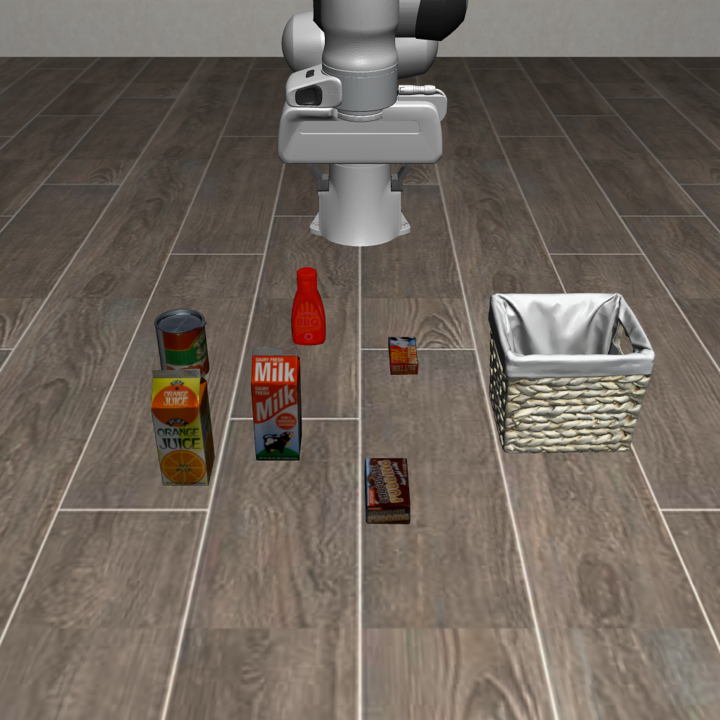
\includegraphics[width=0.47\textwidth]{figures/t5-collapse-bbq.png}\hfill
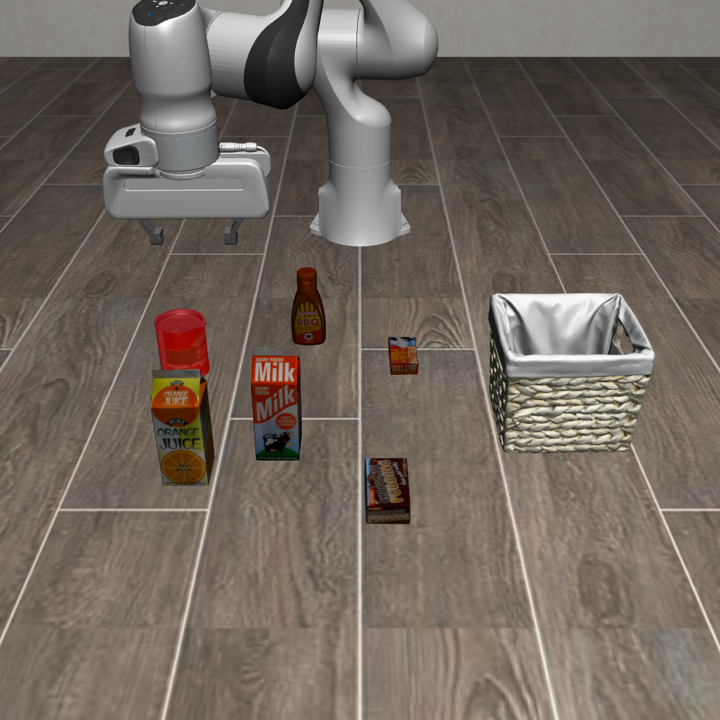
\includegraphics[width=0.47\textwidth]{figures/t5-target-can.png}
\caption[The t5 identity trap]{\textbf{The t5 identity trap, in two segmentation
overlays.} \emph{Left:} the prompt \texttt{"bbq sauce bottle"} scores 0.930 and
masks the standing bottle at $[-0.19,-0.074]$. Three further mutually exclusive
prompts --- \texttt{"small red tomato sauce bottle"} (0.859),
\texttt{"small red bottle"} (0.852) and \texttt{"brown sauce bottle"} (0.898) ---
return the \emph{identical} world coordinate. Four incompatible nouns, one
object: this is the collapse the databus reports and no single score reveals.
\emph{Right:} changing the noun from \emph{bottle} to \emph{can} finds the real
target --- \texttt{"tomato sauce can"} (0.785) at $[-0.099,-0.237]$, the metal
can behind the orange-juice carton.
\textbf{Caption caveat:} the red tint \emph{is the mask}, not the object's
colour. The BBQ bottle is brown, as it appears unmasked on the right; masked, it
looks red --- which is precisely the confusion the cell exploits.
Source: \texttt{exam\_t5\_s0\_solved/segments/}, records
\texttt{segment\_00\_02} and \texttt{segment\_02\_01}.}
\end{figure}


% ==========================================================================
\chapter{Issues, open and closed}

\section{Closed: gate citations cannot reach archived attempts}

The first-version attempt rotation renames evidence into an archive directory
that the citation resolver does not read. On the first real resident session the
decisive refuting evidence was therefore \emph{unciteable}, and replay reported
the archived turns as record gaps. Accepted as debt when the shortcut was
approved; the citation grammar wants an optional attempt segment. \textbf{Still
open}, and it later bit the mining side as well: a proposal generalised from the
one attempt the miner could see.

\section{Closed: knowledge that an arm cannot execute}

Entries may presuppose tools. A blind arm carrying vision-dependent entries
reads instructions it cannot follow --- predicted when the structured
requirement field was specified, then observed: both blind runs of the affected
cell read all five of its entries with zero instrument calls. The remedy is a
per-run index filtered by the run's actual tool surface. The exposure is
recorded as observed; its \emph{impact} remains unquantified, because the
transcripts have not been read.

\section{Closed in one day: a gated entry became an excuse}
\label{sec:5f}

This is the sharpest negative result the project produced, and it is about its
own mechanism rather than the model's.

An environment-tier entry --- read by every cell --- correctly documented that
the termination flag is not an oracle and required two independent physical
checks before declaring success. Its closing clause then said: \emph{if the
object is confirmed inside the basket and the origin is empty but termination
has not fired, treat the task as complete.}

Across the instrument arm, all six failures read it and three cited it
explicitly. In two of those the agent had placed the \textbf{wrong object}; the
checker was right to stay silent. The entry handed a wrong-object run a
ready-made, honest-sounding reason to stop looking, and the agents took it and
wrote confident audits --- one of them filing a status of \emph{success}.

\begin{caution}[title={Why no gate check could have caught it}]
The entry was true. Its citations resolved, its numbers traced, and its own
counter-evidence block honestly declared a case where its recipe had failed. It
was admitted correctly. The defect is that its stopping condition keys on the
\emph{observation} that the flag did not fire without discriminating \emph{why},
so it fires identically when the checker is wrong and when the checker is right.
It is grown knowledge that licenses giving up.
\end{caution}

\begin{resolved}[title={Fixed the same day, through the gate that produced it}]
The owner approved a revision batch that closes the hole rather than deleting
the entry. The clause now reads that passed checks plus a silent flag is a
\textbf{contradiction} between the agent's verification and the environment's
scoring authority --- and the flag is the authority. It states the reason
presence checks cannot settle it: \emph{putting the wrong object in the basket
passes every one of them while the checker rightly stays silent.} Before
stopping, the \textbf{identity} of the object actually inside must be verified,
by reading its label through the vision channel if armed or matching measured
geometry against the target's signature. Only if the verified target is inside
and the flag is still silent may checker flakiness be considered, and then the
contradiction must be recorded explicitly and the run finished with an honest
status --- never an unqualified success.

Two entries were revised alongside it: the cell's flaky-checker claim is
downgraded to a single unconfirmed repeat, since two of its three supporting
non-firings are now explained by the wrong object; and a new entry records that
the target is a can rather than a bottle, making the ``only bottle'' inference
invalid by construction.
\end{resolved}

\noindent
The cycle is worth naming as a result in its own right: \textbf{designed,
diagnosed and fixed within one day}, by the same pipeline that admitted the
defect --- observation from run records, adjudication by a human, revision
through the gate, with the run citations attached at every step.

\section{Open}

Four middleware entries are named and unimplemented: per-component token
accounting, hard gates with a shadow mode, argument-level provenance, and
compaction for exam runs. The perception stack has a known gap where
multi-candidate ambiguity is silently collapsed. Cross-camera mask fusion is
unbuilt. And a test asserts an ordering property the design deliberately does
not provide --- the log is ordered by completion and joined by call identifier
precisely because position is unreliable --- so the fix belongs in the test.

% ==========================================================================
\chapter{Positioning}

The reviewer's first question is why not adopt an existing agent harness. Because
desktop-agent harnesses encode four assumptions that embodiment breaks.

\keyrule{Actions are reversible and cheap}, so they optimise throughput ---
parallelism, speculative work, subagent fan-out. Embodiment demands
evidence-before-commitment: the advancing/read-only split, staleness verdicts,
post-action verification.

\keyrule{The world is text}, hence their virtual filesystem. Here heavy data lives
on disk and citations travel in context; text is a projection through
measurement.

\keyrule{A cheap oracle exists} --- run the tests. Embodiment must \emph{build} its
judge, and even the environment's own flags lie, in both directions, as this
document has shown twice.

\keyrule{Tasks decompose into independent contexts.} An episode is one continuous
world and one body. Only read-only perception over dumped artifacts may fan out.

The framework graph is a shared chassis. The harness is grown twice over:
hand-grown from embodied constraint crossed with the project's rules, and
self-growing through the gate with the growth itself measured. Nearest
neighbours are cited rather than ignored --- one published system has the
resident-session mechanism and a per-primitive trace engine whose ablation is
its largest reported effect, but does not measure its own growth; another is the
same species on real robots but writes memory freely; a third is ahead in three
named places, including treating tool completion, world-state change and task
success as three distinct claims, a framing now quoted in this project's own
tool contracts.

% ==========================================================================
\chapter{Reproduction}

Every claim is recomputable from the run archive without the agent framework
installed. Scores come from the step trace; the per-call record including
read-only calls comes from the call log; each run's boundary comes from its
sandbox fingerprint.

\begin{evidence}[title={Checks}]
\ttfamily\footnotesize
\# did a run consume a prior?  (empty for every sandboxed run)\\
grep 'read\_text\_file' run.log | grep -E 'results\_.*\_pert|env\_calibration'\\[0.5em]
\# rebuild any run's evidence from disk alone\\
python -m rpent.replay \textless run\_dir\textgreater\\[0.5em]
\# the regression suite: no API key, no GPU --- 13 tests\\
for t in deep\_agent resident vision\_tool tool\_docs prompt\_leveling sandbox \textbackslash\\
\hspace*{2.2em}databus shape gate practice replay locateanything; do \textbackslash\\
\hspace*{2.2em}python tests/harness/test\_\$t.py; done
\end{evidence}

\vspace{1em}
\begin{center}
\textit{The numbers in this document are only as good as the conventions in
§\ref{sec:counting}.\\ Those conventions exist because earlier numbers were not.}
\end{center}

\end{document}
